\chapter{トレースログ可視化ツール(TLV)}
\section{TLVにおける汎用性と拡張性}
TLVは、汎用性と拡張性を実現することを目標としている。

汎用性とは、可視化表示したいトレースログの形式を制限しないことであり、
可視化表示の仕組みをトレースログの形式に依存させないことによって実現す
る。具体的には、まず、トレースログを抽象的に扱えるように、トレースログ
を一般化した標準形式トレースログを定義する。そして、任意の形式のトレー
スログを標準形式トレースログに変換する仕組みを、変換ルールとして形式化
する。変換ルールの記述で任意のトレースログが標準形式トレースログに変換
することができるため、あらゆるトレースログの可視化に対応することが可能
となる。

拡張性とは、トレースログに対応する可視化表現をユーザレベルで拡張できる
ことを表し、トレースログから可視化表示を行う仕組みを抽象化し、それを可
視化ルールとして形式化して定義することで実現する。可視化ルールを記述す
ることにより、トレースログ内の任意の情報を自由な表現方法で可視化するこ
とが可能になる。


\section{標準形式トレースログ}\label{sec:log}
\subsection{トレースログの抽象化}
標準形式トレースログを提案するにあたり、トレースログの抽象化を行った。

トレースログを、時系列にイベントを記録したものである。
イベントとはイベント発生源の属性の変化、イベント発生源の振る舞いと考え
た。ここで、イベント発生源をリソースと呼称し、固有の識別子をもつものと
する。つまり、リソースとは、イベントの発生源であり、名前を持ち、固有の
属性をもつものと考えることができる。

リソースは型により属性、振る舞いを特徴付けられる。ここでリソースの型を
リソースタイプと呼称する。

属性は、リソースが固有にもつ文字列、数値、真偽値で表されるスカラーデー
タとし、振る舞いはリソースの行為であるとする。

リソースタイプとリソースの関係は、オブジェクト指向におけるクラスとオブ
ジェクトの関係に類似しており、属性と振る舞いはメンバ変数とメソッドに類
似している。ただし、振る舞いはリソースのなんらかの行為を表現しており、
メソッドの、メンバ変数を操作するための関数や手続きを表す概念とは異なる。

主に、振る舞いは、属性の変化を伴わないイベントを表現するために用いる。
振る舞いは任意の数のスカラーデータを引数として受け取ることができ、これ
は、図形描画の際の条件、あるいは描画材料として用いられることを想定して
いる。

%% 図\ref{fig:resourceTypeSample}と図\ref{fig:resourceSample}に、リソース
%% タイプとリソースを図で表現した例を示す。さらに、図
%% \ref{fig:resourceTypeSampleByTask}に、RTOS(Real-time operating system)
%% におけるタスクの概念をリソースタイプとして表現した例を、図
%% \ref{fig:resourceSampleByTask}に、リソースタイプTaskのリソースの例とし
%% てMainTaskを示す。

トレースログの抽象化を以下にまとめる。

\begin{description}
\item[トレースログ] \mbox{} \\
時系列にイベントを記録したもの。
\item[イベント] \mbox{} \\
リソースの属性の値の変化、リソースの振る舞い。
\item[リソース] \mbox{} \\
イベントの発生源。固有の名前、属性をもつ。
\item[リソースタイプ] \mbox{} \\
リソースの型。リソースの属性、振る舞いを特徴付ける。
\item[属性] \mbox{} \\
リソースが固有にもつ情報。文字列、数値、真偽値のいずれかで表現されるスカラーデータで表される。
\item[振る舞い] \mbox{} \\
リソースの行為。主に属性の値の変化を伴わない行為をイベントとして記録するために用いることを想定している。
振る舞いは任意の数のスカラーデータを引数として受け取ることができる。
\end{description}

%% \begin{figure}[p]
%% \begin{tabular}{cc}
%% \begin{minipage}{0.5\hsize}
%% \begin{center}
%% \includegraphics[scale=0.5]{resourceTypeSample.eps}
%% \caption{リソースタイプ}
%% \label{fig:resourceTypeSample}
%% \end{center}
%% \end{minipage}
%% \begin{minipage}{0.5\hsize}
%% \begin{center}
%% 
\includegraphics[scale=0.5]{resourceSample.eps}
%% \caption{リソース}
%% \label{fig:resourceSample}
%% \end{center}
%% \end{minipage}
%% \end{tabular}
%% \end{figure}

%% \begin{figure}[p]
%% \begin{tabular}{ccc}
%% \begin{minipage}{0.35\hsize}
%% \begin{center}
%% 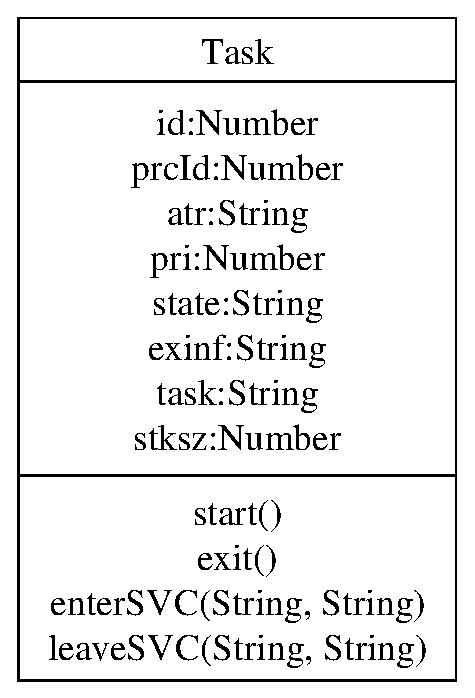
\includegraphics[scale=0.5]{resourceTypeSampleByTask.eps}
%% \caption{タスクをリソースタイプTaskとして表現した例}
%% \label{fig:resourceTypeSampleByTask}
%% \end{center}
%% \end{minipage}
%% \begin{minipage}{0.25\hsize}
%% \mbox{}\\
%% \end{minipage}
%% \begin{minipage}{0.3\hsize}
%% \begin{center}
%% 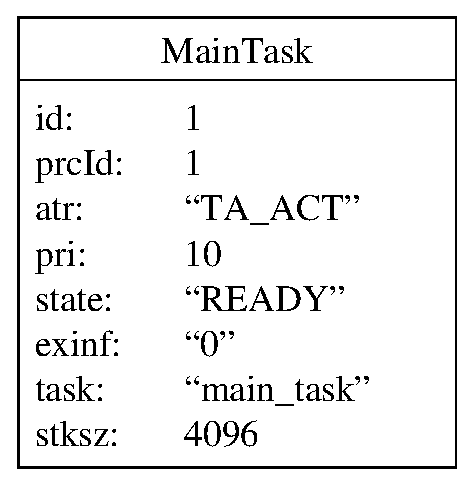
\includegraphics[scale=0.5]{resourceSampleByTask.eps}
%% \caption{リソースタイプTaskのリソースMainTaskの例}
%% \label{fig:resourceSampleByTask}
%% \end{center}
%% \end{minipage}
%% \end{tabular}
%% \end{figure}

\subsection{標準形式トレースログの定義}

本小節では、前小節で抽象化したトレースログを、標準形式トレースログとし
て形式化する。標準形式トレースログの定義は、EBNF(Extended Backus Naur
Form)および終端記号として正規表現を用いて行う。正規表現はスラッシュ記号
({\tt /})で挟むものとする。

前小節によれば、トレースログは、時系列にイベントを記録したものであるの
で、1つのログには時刻とイベントが含まれるべきである。トレースログが記
録されたファイルのデータを\verb|TraceLog|、\verb|TraceLog|を改行記号で
区切った1行を\verb|TraceLogLine|とすると、これらは次のEBNFで表現される。

\begin{EBNF}
TraceLog = { TraceLogLine,"\n" };
TraceLogLine = "[",Time,"]",Event;
\end{EBNF}

\verb|TraceLogLine|は"\verb|[|","\verb|]|"で時刻を囲み、その後ろにイベントを記述するものとする。

時刻は\verb|Time|として定義され、次に示すように数値とアルファベットで構成するものとする。

\begin{EBNF}
Time = /[0-9a-Z]+/;
\end{EBNF}

アルファベットが含まれるのは、10進数以外の時刻を表現できるようにするた
めである。これは、時刻の単位として「秒」以外のもの、たとえば「実行命令
  数」などを表現できるように考慮したためである。この定義から、時刻には、
2進数から36進数までを指定できることがわかる。

前小節にて、イベントを、リソースの属性の値の変化、リソースの振る舞いと
抽象化した。そのため、イベントを次のように定義した。

\begin{EBNF}
Event = Resource,".",(AttributeChange|BehaviorHappen);
\end{EBNF}

{\tt Resource}はリソースを表し、{\tt AttributeChange}は属性の値の変化イ
ベント、{\tt BehaviorHappen}は振る舞いイベントを表す。リソースはリソー
ス名による直接指定、あるいはリソースタイプ名と属性条件による条件指定の
2通りの指定方法を用意した。

リソースの定義を次に示す。

\begin{EBNF}
Resource = ResourceName
         | ResourceTypeName,"(",AttributeCondition,")";
ResourceName = Name;
ResourceTypeName = Name;
Name = /[0-9a-Z_]+/;
\end{EBNF}

リソースとリソースタイプの名前は数値とアルファベット、アンダーバーで構成されるとした。
{\tt AttributeCondition}は属性条件指定記述である。
これは次のように定義する。

\begin{EBNF}
AttributeCondition = BooleanExpression;
BooleanExpression = Boolean
   |ComparisonExpression
   |BooleanExpression,[{LogicalOpe,BooleanExpression}]
   |"(",BooleanExpression,")";
ComparisonExpression = AttributeName,ComparisonOpe,Value;
Boolean = "true"|"false";
LogicalOpe = "&&"|"||";
ComparisonOpe = "=="|"!="|"<"|">"|"<="|">=";
\end{EBNF}

属性条件指定は、論理式で表され、命題として属性の値の条件式を、等価演算子や比較演算子を用いて記述できるとした。

{\tt AttributeName}はリソースの名前であり、リソース名やリソースタイプ名と同様に、次のように定義する。

\begin{EBNF}
AttributeName = Name;
\end{EBNF}

イベントの定義にて、\verb|AttributeChange|は属性の値の変化を、\verb|BehaviorHappen|は振る舞いを表現しているとした。
これらは、リソースとドット"\verb|.|"でつなげることでそのリソース固有のものであることを示す。
リソースの属性の値の変化と振る舞いは次のように定義した。

\begin{EBNF}
AttributeChange = AttributeName,"=",Value;
Value = /[^"\\]+/;
BehaviorHappen =  BehaviorName,"(",Arguments,")";
BehaviorName = Name;
Arguments = [{Argument,[","]}];
Argument = /[^"\\]*/;
\end{EBNF}

属性の変化イベントは、属性名と変化後の値を代入演算子でつなぐことで記述し、振る舞いイベントは、振る舞い名に続けてカンマで区切った引数を括弧"{\tt ()}"で囲み記述するとした。


\subsection{標準形式トレースログの例}

前小節の定義を元に記述した、標準形式トレースログの例を表\ref{standartFormatTraceLogSample}に示す。

\begin{File}{標準形式トレースログの例}{standartFormatTraceLogSample}
[2403010]MAIN_TASK.leaveSVC(ena_tex,ercd=0)
[4496099]MAIN_TASK.state=READY
[4496802]TASK(state==RUNNING).state=READY
\end{File}

1行目がリソースの振る舞いイベントであり、2行目、3行目が属性の値の変化イベントである。
1行目の振る舞いイベントには引数が指定されている。

1行目、2行目はリソースを名前で直接指定しているが、3行目はリソースタイプと属性の条件によってリソースを特定している。

\section{図形データ}\label{subsec:visualization}
\subsection{座標系}

図形を定義する座標系と、表示する座標系は分離して考えるとする。
これにより、図形を表示環境から独立して定義することが可能になる。
図形を定義する座標系をローカル座標系、表示する座標系をデバイス座標系と呼称する。

また、TLVでは、高さと時間を次元に持つ、ワールド座標系という座標系を導入
した。ローカル座標系で定義された図形は、はじめに、ワールド座標系におけ
る、図形を表示すべき時間の領域にマッピングされ、これを表示環境に依存す
るデバイス座標系にマッピングすることで表示する。これにより、図形の表示
領域を、抽象度の高い時刻で指定することが可能になる。ここで、ローカル座
標系からワールド座標系へのマッピングをワールド変換と呼称する。また、表
示する時間の領域を表示期間と呼称する。表示期間は開始時刻と終了時刻で表
される時刻のペアである。

ローカル座標系において、図形の大きさと位置を定義する際は、pixel単位によ
る絶対指定か、ワールド座標系へのマッピング領域に対する割合を\%で指定す
る相対指定かのいずれかを用いる。

図\ref{fig:coordinate}に座標系の例を、図\ref{fig:worldTransform}にワー
ルド変換の例を示す。

\begin{figure}[tb]
\begin{center}
\includegraphics[scale=0.75]{coordinate.eps}
\caption{座標系}
\label{fig:coordinate}
\end{center}
\end{figure}

\begin{figure}[tb]
\begin{center}
\includegraphics[scale=0.75]{worldTransform.eps}
\caption{ワールド変換}
\label{fig:worldTransform}
\end{center}
\end{figure}

\subsection{基本図形と図形、図形群}\label{sec:shape}
可視化表現は、複数の図形を組み合わせることで実現する。
この際、基本となる図形の単位を基本図形と呼称する。

基本図形として扱える形状は楕円、多角形、四角形、線分、矢印、扇形、文字列の7種類とする。
基本図形は、形状や大きさ、位置、塗りつぶしの色、線の色、線種、透明度などの属性を指定して定義する。

複数の基本図形を仮想的にz軸方向に階層的に重ねたものを、単に図形と呼称し、可視化表現の最小単位とする。
図形は、構成する基本図形を順序付きで指定し、名前をつけて定義する。
図形は名前を用いて参照することができ、その際に引数を与えることができるとする。
この際、引数は、図形を構成する基本図形の、任意の属性に割り当てることを想定している。

複数の図形を仮想的にz軸方向に階層的に重ねたものを図形群と呼称する。
図\ref{fig:shapes}に図形と図形群の例を示す。

\begin{figure}[tb]
\begin{center}
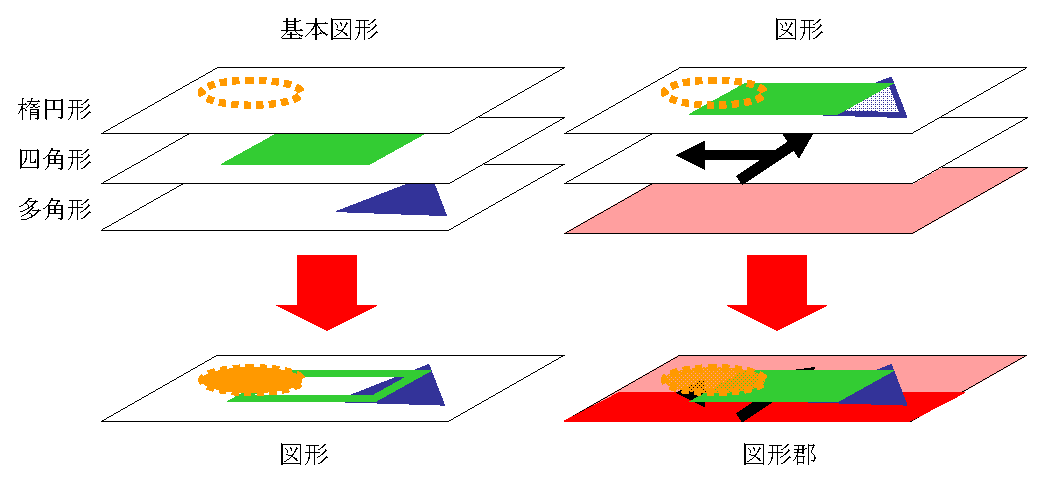
\includegraphics[scale=0.75]{shapes.eps}
\caption{図形と図形群}
\label{fig:shapes}
\end{center}
\end{figure}

\section{図形データとイベントの対応}

本小節では、前小節で述べた可視化表現とトレースログのイベントをどのように対応付けるのかを述べる。

\subsection{開始イベント、終了イベント、イベント期間}
前小節において、可視化表現は、図形をワールド変換を経て表示期間にマッピ
ングすることであることを説明した。ここで、表示期間の開始時刻、終了時刻
を、イベントを用いて指定するとする。つまり、指定されたイベントが発生す
る時刻をトレースログより抽出することにより表示期間を決定する。このよう
にして、トレースログのイベントと可視化表現を対応付ける。ここで、開始時
刻に対応するイベントを開始イベント、終了時刻に対応するイベントを終了イ
ベントと呼称し、表示期間をイベントで表現したものをイベント期間と呼称す
る。

\subsection{可視化ルール}

図形群と、そのマッピング対象であるイベント期間を構成要素としてもつ構造体を、可視化ルールと呼称する。
図\ref{fig:timeShape}に、標準形式トレースログを用いてイベント期間を定義した可視化ルールの例を示す。
\begin{figure}[tb]
\begin{center}
\includegraphics[scale=0.9]{timeShape.eps}
\caption{可視化ルール}
\label{fig:timeShape}
\end{center}
\end{figure}
図\ref{fig:timeShape}において、runningShapeを、位置がローカル座標の原点、
大きさがワールド座標系のマッピング領域に対して横幅100\%、縦幅80\%の長方
形で色が緑色の図形とする。この図形を、開始イベント
\verb|MAIN_TASK.state=RUNNING|、終了イベント\verb|MAIN_TASK.state|とな
るイベント期間で表示するよう定義したものが可視化ルール
taskBecomeRunningである。開始イベント\verb|MAIN_TASK.state=RUNNING|は、
リソース\verb|MAIN_TASK|の属性\verb|state|の値が\verb|RUNNING|になった
ことを表し、終了イベント\verb|MAIN_TASK.state|は、リソース
\verb|MAIN_TASK|の属性\verb|state|の値が単に変わったことを表している。

taskBecomeRunningを、表\ref{eventTime}に示すトレースログからイベントを
抽出して表示期間の時刻を決定し、図形のワールド変換を行った結果が図
\ref{fig:timeShape}の右下に示すものである。

\begin{File}{イベント期間を抽出するトレースログ}{eventTime}
[1000]MAIN_TASK.state=RUNNING
[1100]MAIN_TASK.state=WAITING
\end{File}

\section{TraceLogVisualizerの設計}

TLVの主機能は、2つの主たるプロセスと6種の外部ファイルによって実現される。
図\ref{fig:tlv}にTLVの全体像を示す。

2つの主たるプロセスとは、標準形式への変換と、図形データの生成である。標
準形式への変換は、任意の形式をもつトレースログを標準形式トレースログに
変換する処理である。この処理には、外部ファイルとして変換元のトレースロ
グファイル、リソースを定義したリソースファイル、リソースタイプを定義し
たリソースヘッダファイル、標準形式トレースログへの変換ルールを定義した
変換ルールファイルが読み込まれる。

また、図形データの生成は、変換した標準形式トレースログに対して可視化ルー
ルを適用し図形データを生成する処理である。この処理には外部ファイルとし
て可視化ルールファイルが読み込まれる。可視化ルールファイルとは図形と可
視化ルールの定義を記述したファイルである。

TLVは、トレースログとリソースファイルを読み込み、トレースログの対象に対
応したリソースヘッダファイル、変換ルールファイルの定義に従い、標準形式
トレースログを生成する。生成された標準形式トレースログに可視化ルールファ
イルで定義される可視化ルールを適用し図形データを生成した後、画面に表示
する。

生成された標準形式トレースログと図形データは、TLVデータとしてまとめられ
可視化表示の元データとして用いられる。TLVデータはTLVファイルとして外部
ファイルに保存することが可能であり、TLVファイルを読み込むことで、標準形
式変換と図形データ生成の処理を行わなくても可視化表示できるようになる。

図\ref{fig:TLVscreenshot}に、TLVのスクリーンショットを示す。

\begin{figure}[!t]
\begin{center}
\includegraphics[scale=0.7]{tlv.eps}
\caption{TLVの全体像}
\label{fig:tlv}
\end{center}
\end{figure}

\begin{figure}[!t]
\begin{center}
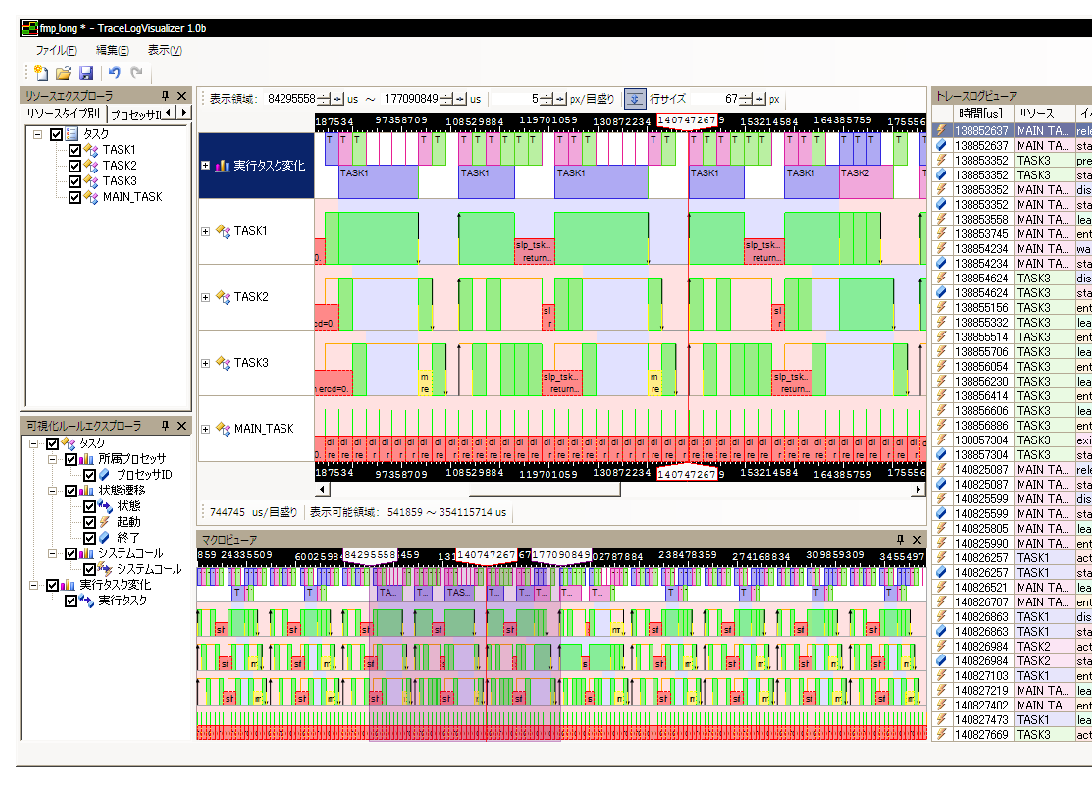
\includegraphics[scale=0.7]{TLVscreenshot.eps}
\caption{TLVのスクリーンショット}
\label{fig:TLVscreenshot}
\end{center}
\end{figure}

%% \subsection{Json}

%% リソースファイル、リソースヘッダファイル、変換ルールファイル、可視化ルールファイルは、Json(JavaScript Object Notation)\cite{Json}と呼ばれるデータ記述言語を用いて記述する。

%% Jsonは、主にウェブブラウザなどで使用されるECMA-262、revision 3準拠のJavaScript(ECMAScript)と呼ばれるスクリプト言語のオブジェクト表記法をベースとしており、RFC 4627としてで仕様が規定されている。
%% JsonはUnicodeのテキストデータで構成され、バイナリデータを扱うことはできない。
%% また、Jsonではシンタックスのみの規定がなされ、セマンティクスは規定されていない。

%% Jsonの特徴は、シンタックスが単純であることである。
%% これは、人間にとっても読み書きし易く、コンピュータにとっても解析し易いことを意味する。
%% また、複数のプログラミング言語でJsonファイルを扱うライブラリが実装されており、異なる言語間のデータ受け渡しに最適である。
%% Jsonが利用可能なプログラミング言語としては、ActionScript, C, C++, C\#, ColdFusion, Common Lisp, Curl, D言語, Delphi, E, Erlang, Haskell, Java, JavaScript (ECMAScript), Lisp, Lua, ML, Objective CAML, Perl, PHP, Python, Rebol, Ruby, Scala, Squeakなどがある。

%% TLVの各ファイルのフォーマットにJsonを採用した理由はこれらの特徴による。
%% シンタックスが単純であることにより、ユーザの記述コスト、習得コストを低減させることができ、また、複数のプログラミング言語でパース可能であることによりファイルに可搬性を持たせることができるからである。

%% Jsonで表現するデータ型は以下のとおりであり、これらを組み合わせることでデータを記述する。
%% \begin{itemize}
%% \setlength{\itemsep}{0.5\itemsep}
%% \item 数値(整数、浮動小数点)
%% \item 文字列(Unicode)
%% \item 真偽値(true、false)
%% \item 配列(順序付きリスト)
%% \item オブジェクト(ディクショナリ、ハッシュテーブル)
%% \item null
%% \end{itemize}

%% Jsonの文法をEBNFと正規表現を用いて説明する。

%% Jsonは、次に示すようにオブジェクトか配列で構成される。

%% \begin{EBNF}
%% JsonText = Object | Array;
%% \end{EBNF}

%% オブジェクトは複数のメンバをカンマで区切り、中括弧で囲んで表現する。
%% メンバは名前と値で構成され、名前のあとにはセミコロンが付く。
%% メンバの名前は値であり、データ型は文字列である。
%% オブジェクトの定義を次に示す。

%% \begin{EBNF}
%% Object = "{",Member,[{",",Member}],"}";
%% Member = String,":",Value;
%% \end{EBNF}

%% 配列は複数の値を持つ順序付きリストであり、値をコンマで区切り、角括弧で囲んで表現する。
%% 次に配列の定義を示す。

%% \begin{EBNF}
%% Array = "[",Value,[{",",Value}],"]";
%% \end{EBNF}

%% 値は、文字列、数値、オブジェクト、配列、真偽値、nullのいずれかである。
%% 文字列はダブルクオーテーションで囲まれたUnicode列である。
%% 数値は10進法表記であり、指数表記も可能である。
%% 値の定義を次に示す。

%% \begin{EBNF}
%% Value = String|Number|Object|Array|Boolean|"null";
%% String = /"([^"\]|\n|\"|\\|\b|\f|\r|\t|\u[0-9a-fA-F]{4})*"/;
%% Boolean = "true"|"false";
%% Number = ["-"],("0"|Digit1-9,[Digit]),[".",Digit],Exp;
%% Exp = ["e",[("+"|"-")],Digit];
%% Digit = /[0-9]+/;
%% Digit1-9 = /[1-9]/;
%% \end{EBNF}

%% 表\ref{JsonObject}にJsonにおけるオブジェクトを定義した例を示す。

%% \begin{FileToPage}{Jsonにおけるオブジェクトを定義した例}{JsonObject}
%% {
%%   "Image":{
%%     "Width":  800,
%%     "Height": 600,
%%     "Title":  "View from 15th Floor",
%%     "Thumbnail":{
%%       "Url":    "http://www.example.com/image/481989943",
%%       "Height": 125,
%%       "Width":  "100"
%%     },
%%     "IDs": [116, 943, 234, 38793]
%%   }
%% }
%% \end{FileToPage}

%% 表\ref{JsonArray}にJsonにおける配列を定義した例を示す。

%% \begin{FileToPage}{Jsonにおける配列を定義した例}{JsonArray}
%% [
%%   {
%%     "City":      "SAN FRANCISCO",
%%     "State":     "CA",
%%     "Zip":       "94107",
%%     "Country":   "US"
%%   },
%%   {
%%     "City":      "SUNNYVALE",
%%     "State":     "CA",
%%     "Zip":       "94085",
%%     "Country":   "US"
%%   },
%%   {
%%     "City":      "HEMET",
%%     "State":     "CA",
%%     "Zip":       "92544",
%%     "Country":   "US"
%%   }
%% ]
%% \end{FileToPage}

\subsection{標準形式トレースログへの変換}\label{convertRule}
標準形式トレースログへの変換は、トレースログファイルを先頭から行単位で
読み込み、変換ルールファイルで定義される置換ルールに従い標準形式トレー
スログに置換していくことで行われる。

リソース属性の遷移に伴うイベントや、元のトレースログに欠落
している情報を補うイベントなど、元のトレースログの情報だけでは判断でき
ないイベントを出力するには、特定時刻における特定リソースの有無やその数、
特定リソースの属性の値などの条件で出力を制御できる必要がある。そのため、
TLVの変換ルールでは、置換する条件の指定と、条件指定の際に用いる情報を置
換マクロを用いて取得できる仕組みを提供している。

標準形式トレースログに含まれるリソースは、リソースファイルで定義されて
いなければならない。リソースファイルには、各リソースについて、その名前
とリソースタイプ、必要であれば各属性の初期値を定義する。
また、その際に使用
されるリソースタイプはリソースヘッダファイルで定義されていなければなら
ない。リソースヘッダファイルには各リソースタイプについて、その名前と属
性、振る舞いの定義を記述する。

リソースヘッダ、変換ルール、可視化ルールは可視化するターゲット毎に用意する。
その際のターゲットはリソースファイルに記述する。

\subsection{図形データの生成}\label{visualizeRule}
標準形式変換プロセスを経て得られた標準形式トレースログは、可視化ルール
を適用され図形データを生成する。ここで、図形データとは、ワールド変換が
行われた全図形のデータを指す。可視化ルールは可視化ルールファイルとして
与えられ、適用する可視化ルールはリソースファイルに記述する。

図形データの生成方法は、標準形式トレースログを一行ずつ可視化ルールのイ
ベント期間と一致するか判断し、一致した場合にその可視化ルールの表示期間
をワールド変換先の領域として採用しワールド変換することで行われる。

\section{TraceLogVisualizerのその他の機能}

本節では、標準形式変換と可視化データ生成の他にTLVが備える機能について詳述する。

\subsection{マーカー}
TLVでは、可視化表示部にマーカーと呼ぶ印を指定の時刻に配置することができる
注目するべきイベントの発生時刻にマーカーを配置することで、可視化表示内容の理解を補助することができる。

マーカーとマーカーの間には、その間の時間が表示されるので、ソフトウェアの計測を行うことができる。
マーカーには名前を付けることができ、色の指定が可能である。
また、マーカーはマウス操作で選択することができ、拡大縮小などの各種操作に利用される。
マーカーは階層構造で管理し、階層ごとに表示の切り替え、マーカー間時間の表示などを行うことができる。

\subsection{可視化表示部の制御}

可視化表示ツールでは、可視化表示部を制御する操作性が使い勝手に大きく影響するため、TLVでは目的や好みに合わせて様々な操作で制御を行えるようにした。
TLVでは、可視化表示部の制御として、表示領域の拡大縮小、移動を行うことができる。
これらの操作方法として、キーボードによる操作、マウスによる操作、値の入力による操作の3つの方法を提供した。

マウスによる操作は、クリックによる操作、ホイールによる操作、選択による操作がある。
クリックによる操作はカーソルを虫眼鏡カーソルに変更してから行う。
左クリックでカーソル位置を中心に拡大、右クリックで縮小を行う。
また、左ダブルクリックを行うことでクリック箇所が中心になるように移動する。
ホイールによる操作は、コントロールキーを押しながらホイールすることで移動を行い、シフトキーを押しながら上へホイールすることでカーソル位置を中心に拡大、下へスクロールすることで縮小する。
選択による操作では、マウス操作により領域を選択し、その領域が表示領域になるように拡大する。

キーボードによる操作は、可視化表示部において方向キーを押すことで行い、微調整するのに適している。
左キーで表示領域を左に移動し、右キーで右に移動する。
上キーでカーソル位置、または選択されたマーカーを中心に表示領域を縮小し、下キーで拡大する。

値の入力による操作では、より詳細な制御を行うことができる。
可視化表示部の上部にはツールバーが用意されており、そこで表示領域の開始時刻と終了時刻を直接入力することができる。

\subsection{マクロ表示}

TLVの要求分析を行った際、可視化表示部で拡大した場合に全体の内どの領域を表示しているのかを知りたいという要求があった。
そのため、TLVでは、マクロビューアというウィンドウを実装した。

マクロビューアでは、トレースログに含まれるイベントの最小時刻から最大時刻までを常に可視化表示しているウィンドウで、可視化表示部で表示している時間を半透明の色で塗りつぶして表示する。
塗りつぶし領域のサイズをマウスで変更することができ、それに対応して可視化表示部の表示領域を変更することができる。

マクロビューアでは可視化表示部と同じように、キーボード、マウスにより拡大縮小、移動の制御を行うことができる。

\subsection{トレースログのテキスト表示}

TLVでは、標準形式トレースログをテキストで表示するウィンドウを実装した。
ここでは、トレースログの内容を確認することができる。

可視化表示部とテキスト表示ウィンドウは連携しており、テキスト表示ウィンドウでマウスを移動すると、カーソル位置にあるトレースログの時刻にあわせて可視化表示部のカーソルが表示されたり、ダブルクリックすることで対応する時刻に可視化表示部を移動することができる。
また、可視化表示部でダブルクリックすることで、ダブルクリック位置にある図形に対応したトレースログが、テキスト表示ウィンドウの先頭に表示されるようになっている。

\subsection{可視化表示項目の表示非表示切り替え}

TLVでは、可視化表示する項目を可視化ルールにより変更、追加することができるが、それらの表示を可視化ルールやリソースを単位で切り替えることができる。
これらの操作は、リソースウィンドウと可視化ルールウィンドウで行う。
リソースウィンドウではリソースファイルで定義されたリソースを、リソースタイプやグループ化可能な属性毎にツリービュー形式で表示しており、チェックの有無でリソース毎に表示の切り替えを行える。
同じように、可視化ルールウィンドウでは、可視化ルールごとに表示の切り替えを行える。

\section{本OJLで追加した機能}
本OJLで追加したその他の機能について述べる。

\subsection{スクリプト拡張機能}
\sref{convertRule}、
\sref{visualizeRule}で述べた変換・可視化ルールでは記述できない複雑な可視化を実現するためのスクリプト拡張機能を追加した。

詳しくは、\ref{ch:se}章で述べる。


\subsection{タイトルバーに表示中のログファイル名・リソースファイル名を表示}
トレースログを開いた直後はタイトルバーに「新規トレースログ」と表示していた。
しかし、どのトレースログを可視化したのが分かりにくいとよう要望があった。

そこで、
タイトルバーに、開いているログファイル名とリソースファイル名を表示するように変更した。

\subsection{リロード機能}
変換ルール・可視化ルールを記述している際に、
記述を変更するたびにトレースログを開き直す必要があり不便だ、という要望があった。

そこで、
現在開いているトレースログを再度、変換・可視化を行なう
リロードボタンを追加した。

\subsection{ドラッグによる表示範囲移動}
表示範囲の移動は、シフト+マウスホイールかスクロールバーのクリックによっ
て行なっていた。しかし、マウスのドラッグによっても表示範囲を移動させた
いという要望があた。

そこで、ドラッグによっても表示範囲を移動させれるように変更した。

\subsection{時刻表示のカンマ区切り}
可視化ウインドウの時刻表示が、カンマ区切りになっておらず、読みづらとい
う要望があった。

そこで、時刻の基数が10の場合は、3桁ごとにカンマで区切るように変更した。

\subsection{マクロビューの拡大表示}
長いトレースログの場合、マクロビューの表示が細かくなりすぎて、可視化範
囲の選択が難しいので、改善して欲しいという要望があった。

そこで、マクロビューでシフト+マウスホイールを行なった場合、
マクロビューの表示を拡大・縮小するように変更した。
